\documentclass[a4paper]{jpconf}
\usepackage{graphicx}

\begin{document}
\title{AutoPyFactory: A Scalable Flexible Pilot Factory Implementation}

\author{J. Caballero$^1$, J. Hover $^1$, P. Love$^2$, G. Stewart$^3$}

\address{$^1$ Brookhaven National Laboratory, PO BOX 5000 Upton, NY 11973, USA}
\address{$^2$ Department of Physics, Lancaster University, Lancaster, LA1 4YB, UK }
\address{$^3$ Department of Physics and Astronomy, University of Glasgow, Glasgow G12 8QQ, UK}

\ead{jcaballero@bnl.gov}

\begin{abstract}
The ATLAS experiment at the CERN LHC is one of the largest users of grid computing
infrastructure, which is a central part of the experiment's computing operations.
Considerable efforts have been made to use grid technology in the most efficient
and effective way, including the use of a pilot job based workload management framework.
In this model the experiment submits 'pilot' jobs to sites without payload. When these
jobs begin to run they contact a central service to pick-up a real payload to execute.
The first generation of pilot factories were usually specific to a single VO, and were
bound to the particular architecture of that VO's distributed processing. A second
generation provides factories which are more flexible, not tied to any particular VO,
and provide new or improved features such as monitoring, logging, profiling, etc.
In this paper we describe this key part of the ATLAS pilot architecture, a second
generation pilot factory, AutoPyFactory.
AutoPyFactory has a modular design and is highly configurable. It is able to send
different types of pilots to sites and exploit different submission mechanisms and queue
characteristics. It is tightly integrated with the PanDA job submission framework,
coupling pilot flow to the amount of work the site has to run. It gathers information
from many sources in order to correctly configure itself for a site, and its decision logic
can easily be updated.
Integrated into AutoPyFactory is a flexible system for delivering both generic and
specific job wrappers which can perform many useful actions before starting to run
end-user scientific applications, e.g. validation of the middleware, node profiling
and diagnostics, and monitoring.
AutoPyFactory now also has a robust monitoring system and we show how this has helped
establish a reliable pilot factory service for ATLAS.
\end{abstract}


\section{Introduction}

LHC experiments have adopted jobs workflows based on pilots systems.
Even tought the particular implementation of these pilot-based architectures may vary 
between different VOs, the physolophy is the same. 

Generic multipurpose pilot jobs are submitted to sites without payload. 
Only when these jobs begin to run on a grid resource they contact a central VO service 
to pick-up a real payload (as an end-user job) and executes it.
Using these pilot-based workflows helps to improve job reliability,
optimize resources utilization, allows for oportunistics resources usage, 
and mitigates many of the problems associated with the inhomogeneities found on the grid.

Therefore, VO's need for a reliable, robust but scalable framework
capable of managing the automatic flow of pilots to remote Grid resources
accordingly with the load of payload jobs.
These pilot frameworks need to address the different policies that the VOs
implement to handle the different types of payload flavors.

AutoPyFactory is one of these pilot frameworks.


\section{Architecture}


AutoPyFactory runs as a single process,
launching a separate thread for each internal workflow (known as APFQueue).
Each one of these APFQueues typically serves for a single job queue, 
as it is defined in the VO Workload Management WMS service, 
and delivers pilots to a single batch queue,
either local o remotely. 


The behavior of these AutoPyFactory workflows, or APFQueues,
is determined by the combination of a set of plug-ins, 
invoked in a fixed order, 
in a loop,   
each one in charge of the performance of a very well defined action.


These steps can be summarized as follows:
\begin{itemize}
    \item Retrieves possible extra configuration information from an external source 
          and merges it with the one from the local configuration files.
    \item Inspects the VO WMS service to query for end-users jobs and their state.
    \item Inspects the submission system to query how many pilots are already running or still idle.
    \item Makes a decission based on that information, implementing a given algorithm. 
    \item Submits as many new pilots as needed, accordingly with the decision made by the previous step.
\end{itemize}

\subsection{AutoPyFactory internal nomenclature}

The communication between different modules in AutoPyFactory 
is possible thanks to its internal nomenclature.
A set of generic variables with an specific meaning which all components 
understand, allowing them to work together. 
Table 1 and Table 2 show the AutoPyFactory names for the
possible states in the batch submission system. 

\begin{table}
   \begin{center}
      \begin{tabular}{l l}
         \hline
         \textbf{AutoPyFactory status} & \textbf{Description} \\ 
         \hline
         pending      &     job is queued (somewhere) but not running yet.      \\  
         running      &     job is currently active (run + stagein + stageout)  \\ 
         error        &     job has been reported to be in an error state       \\ 
         suspended    &     job is active, but held or suspended                \\ 
         done         &     job has completed                                   \\ 
         unknown      &     unknown or transient intermediate state             \\ 
         \hline
      \end{tabular}
   \end{center}
   \caption{Batch submit system primary AutoPyFactory job status}
   \label{job secondary status}
\end{table}

\begin{table}
   \begin{center}
      \begin{tabular}{l l}
         \hline
         \textbf{AutoPyFactory status} & \textbf{Description}  \\ 
         \hline
         transferring  &     stagein + stageout  \\ 
         stagein       &                         \\ 
         stageout      &                         \\ 
         failed        &     (done - success)    \\ 
         success       &     (done - failed)     \\ 
         \hline
      \end{tabular}
   \end{center}
   \caption{Batch submit system secondary AutoPyFactory job status} 
   \label{job secondary status}
\end{table}

Table 3 shows the list of AutoPyFactory names and their meaning 
for the possible states in the WMS system.

\begin{table}
   \begin{center}
      \begin{tabular}{l l}
         \hline
         \textbf{AutoPyFactory status} & \textbf{Description} \\
         \hline
         notready &     job created in the WMS service, but not ready yet for execution\\ 
         ready    &     job ready to be picked up and start execution                  \\ 
         running  &     job is currently running                                       \\ 
         done     &     job has finished with success                                  \\ 
         failed   &     job has finished with no success                               \\ 
         \hline
      \end{tabular}
   \end{center}
   \caption{WMS service AutoPyFactory job status}
   \label{wms job status}
\end{table}

\subsection{Plug-ins design}

AutoPyFactory can serve to different queues in different ways 
thanks to its modular design based on plug-ins. 
Plug-ins serve two purposes. 
They interact with the external services, like the VO WMS service or the batch submission system,
and they translate the information retrieved by those services into the internal AutoPyFactory nomenclature.
There are currently 5 types of plug-ins:


\subsubsection{Configuration Plug-in:}

Retrieves extra configuration content from remote sources 
(as an URL with the actual configuration file, or a web service with an API providing for the configuration content)
and merge them with the local configuration content.
An example of a configuration plugi-in queries the PanDA SchedConfig service.


\subsubsection{WMS Status Plug-in:}
Queries the VO WMS system, 
retrieving information about the number of jobs in different status (ready, running, finished...) per queue.
This information is converted internally into the AutoPyFactory nomenclature.
An example of a WMS Status plug-in queries the PanDA API.
Another example is a plug-in querying a local Condor pool and interpreting the output as end-user jobs.
Table 4 shows an example of mapping between the VO WMS service 
(PanDA in this case)
and the internal AutoPyFactory nomenclature.

\begin{table}
   \begin{center}
      \begin{tabular}{l l}
         \hline
         \textbf{Panda Status} & \textbf{AutoPyFactory Status}       \\
         \hline
         pending       & notready  \\ 
         defined       & notready  \\ 
         assigned      & notready  \\ 
         waiting       & notready  \\ 
         activated     & ready     \\ 
         starting      & running   \\ 
         sent          & running   \\ 
         running       & running   \\ 
         holding       & running   \\ 
         transferring  & running   \\ 
         finished      & done      \\ 
         failed        & failed    \\ 
         cancelled     & failed    \\ 
         \hline
      \end{tabular}
   \end{center}
   \caption{Mapping between PanDA status and AutoPyFactory WMS job status}
   \label{translation}
\end{table}


\subsubsection{Batch Status Plug-in:}
Queries the batch system being used to submit the jobs (or pilots) to the grid resources,
to determine how many previously submitted jobs are already being executed and how many are still idle.
This information is used to avoid submitting an unnecesary number of extra new jobs, 
which could cause from bottlenecks and inefficiencies on the overall algorithm, to severe damage on remote Grid services.
An example is a module querying the condor queues.
Tables 5 and 6 show two example of mappings between the external services
and the internal AutoPyFactory nomenclature.

\begin{table}
   \begin{center}
      \begin{tabular}{l l}
         \hline
         \textbf{Condor Local Status}  & \textbf{AutoPyFactory Status}       \\ 
         \hline
         Unexpanded (the job has never run)    &  pending     \\
         Idle                                  &  pending     \\
         Running                               &  running     \\
         Removed                               &  done        \\
         Completed                             &  done        \\
         Held                                  &  suspended   \\
         Transferring Output                   &  running     \\
         \hline
      \end{tabular}
   \end{center}
   \caption{Mapping between condor status and AutoPyFactory batch job status}
   \label{translation}
\end{table}

\begin{table}
   \begin{center}
      \begin{tabular}{l l}
         \hline
         \textbf{Globus status Status}   & \textbf{AutoPyFactory status}       \\ 
         \hline
         PENDING       &   pending    \\
         ACTIVE        &   running    \\
         FAILED        &   done       \\
         DONE          &   done       \\
         SUSPENDED     &   suspended  \\
         UNSUBMITTED   &   pending    \\
         STAGE\_IN     &   running    \\
         STAGE\_OUT    &   running    \\
         \hline
      \end{tabular}
   \end{center}
   \caption{Mapping between globus status and AutoPyFactory batch job status}
   \label{translation}
\end{table}


\subsubsection{Scheduler Plugin-in:}
It is the component in charge of making a decision based on the information provided by the two Status plug-ins. 
It implements a given algorithm to decide how many new jobs (or pilots) should be submitted next cyle. 
A typical algorithm calculates the number of new jobs based on the number of end-user jobs in a ready status in the VO WMS service, 
with some constrains to prevent the submission of an excesively high number of jobs, 
or to eventually keep a minimum number of submissions per cycle. 
Another algorithm could just submit always a fixed number of jobs.

\begin{figure}
\centering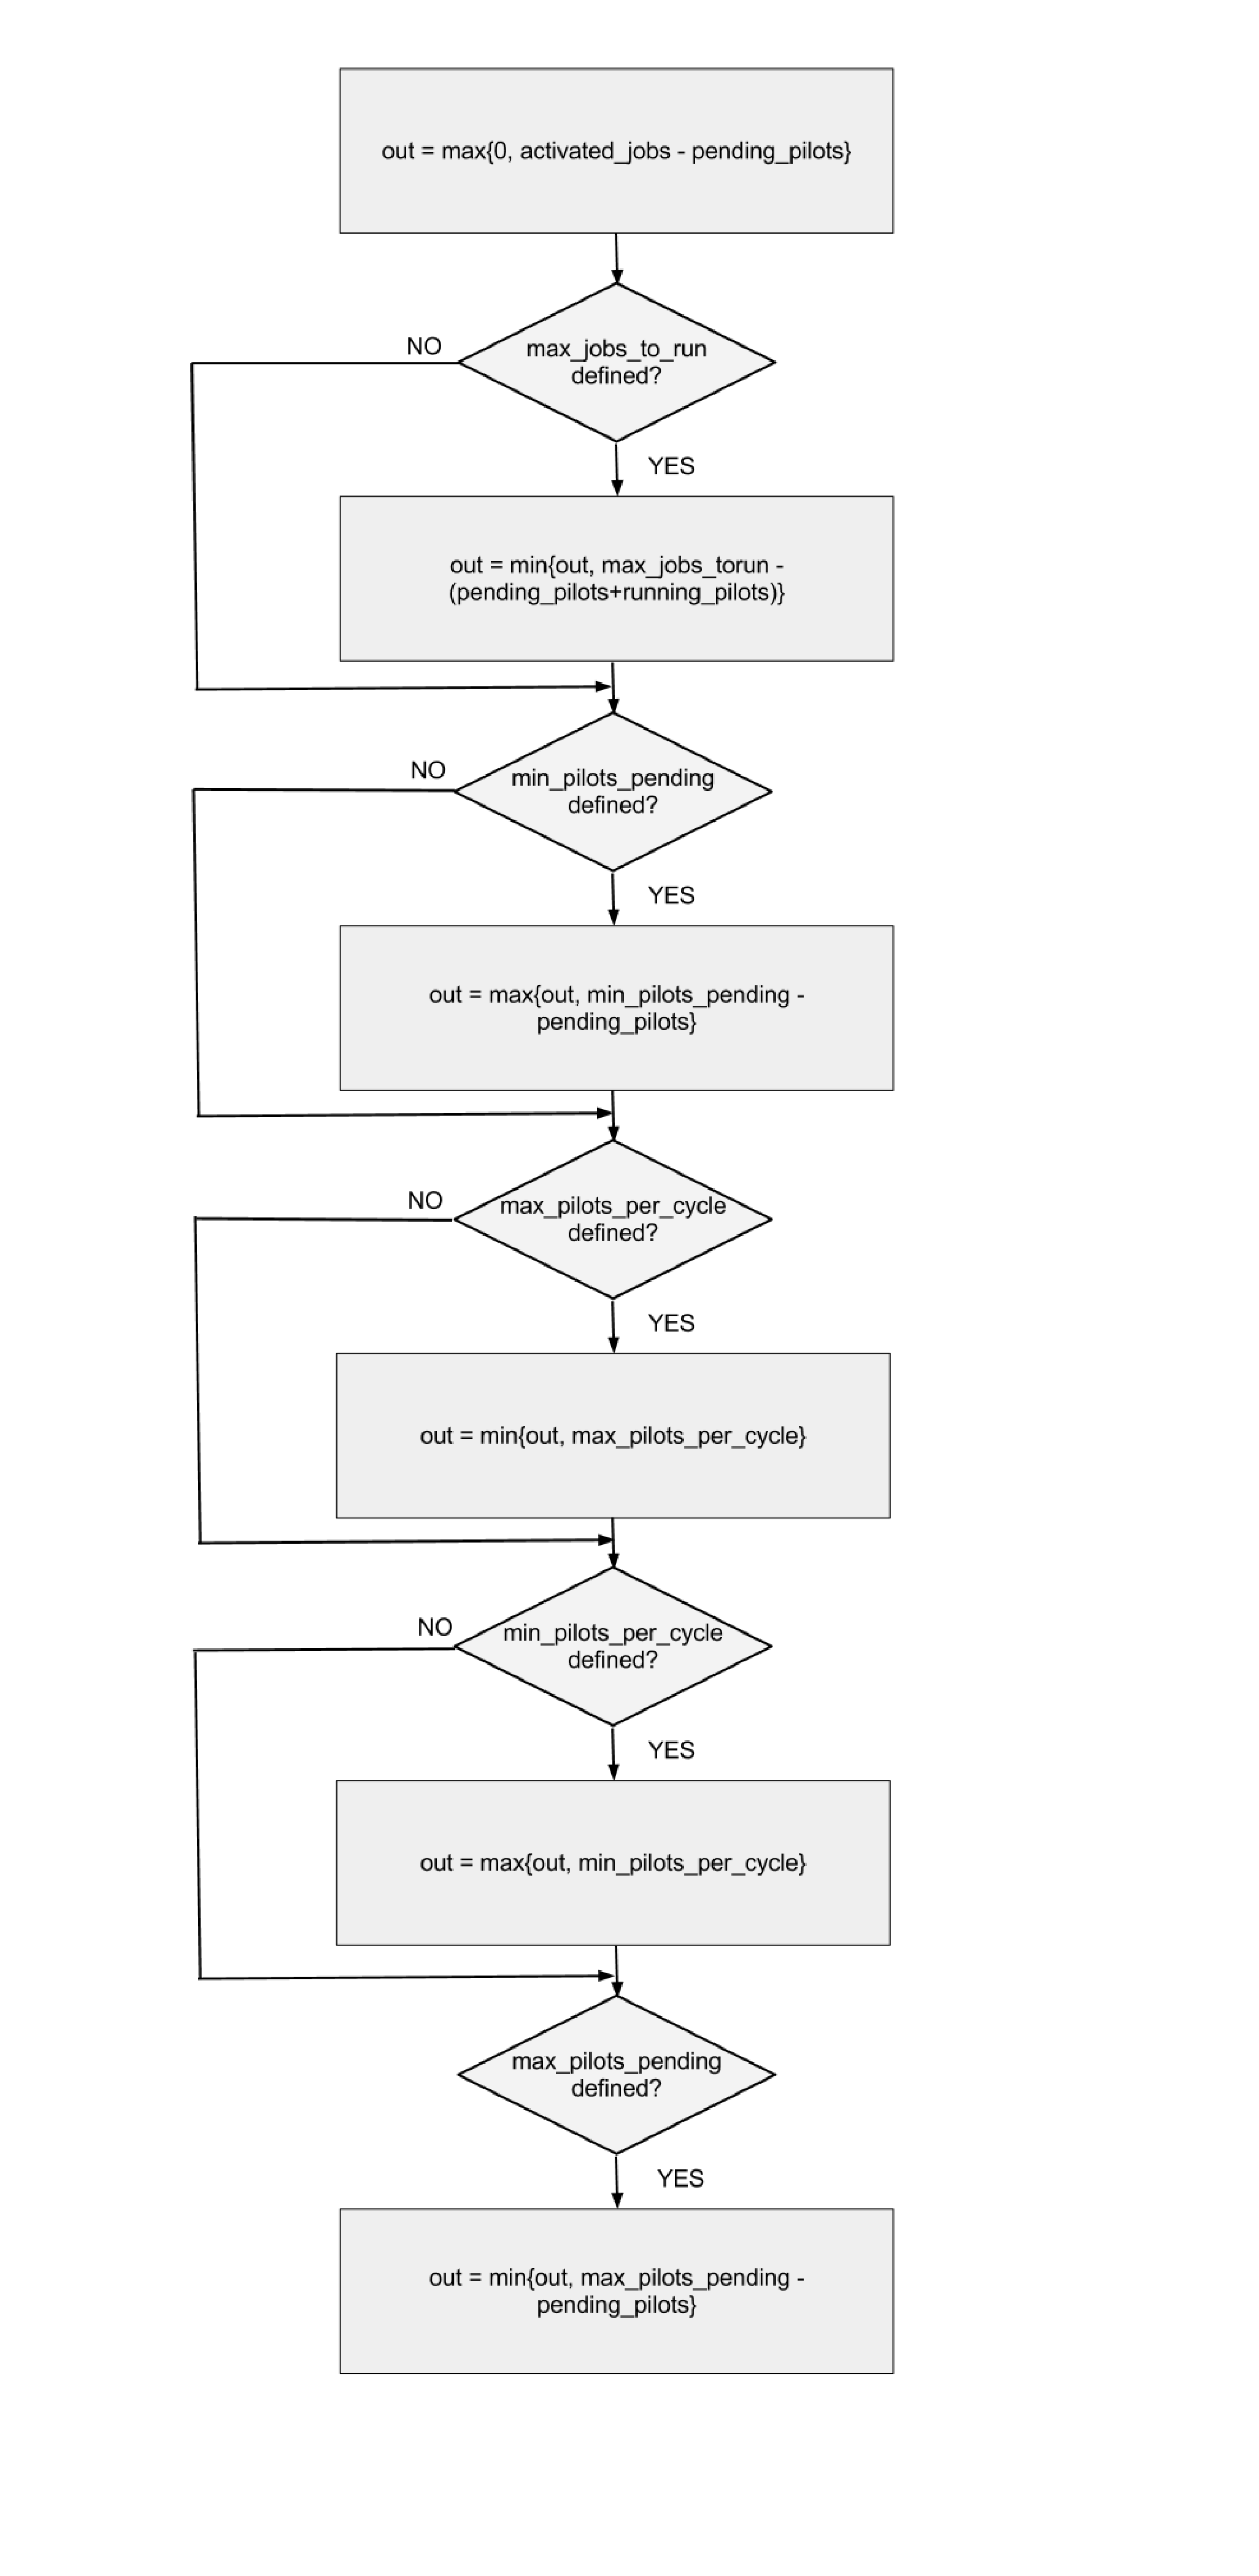
\includegraphics[width=0.7\textwidth]{activated}
\caption{Activated algorithm}
\label{activated}
\end{figure}

\subsubsection{Execution Plug-in:}
It is the component in charge of submitting new jobs (or pilots), 
based on the decision made by the Scheduler plug-in. 
Examples of these execution plugins can submit jobs remotely to a Grid resources using different protocols 
(such as GRAM2, GRAM5, or CREAM),
to a Clould Computing resources (using the Amazon EC2 protocol), 
or to a local Condor pool.


\subsection{Usage}

The normal usage, as explained above, 
makes use of a single set of 5 plug-ins per workflow. 
Typically, each APFQueue will serve one queue as it is defined in the WMS service, 
and will submit pilots to a queue as defined in the batch system. 
This allows for many-to-many combinations, each one served by one APFQueue in a single thread. 

However, more complex workflows can be achieved by the combination of two APFQueues working together.

\subsubsection{Cloud Computing with AutoPyFactory:}
The combination of two APFQueues can allow using Cloud Computing resources. 
For this to happen, the configuration of both APFQueues is like this:

\begin{itemize}
\item First APFQueue: 
the WMS Status plug-in queries the VO WMS service, and the Execution Plugin submits jobs  to a local Condor pool.
This Condor pool can have many Worker Nodes, or zero. 
In the latter case, all submitted jobs will remain in idle status. 
\item Second APFQueue: 
the WMS Status plug-in queries this local condor pool, 
and gives to idle jobs in queue the same meaning that jobs ready in an VO WMS service. 
The Execution Plug-in then submits Virtual Machine instantiation orders (to an Amazon EC2-like resource, for example). 
The middleware pre-installed on these Virtual Machines, 
beside Grid middleware and any particular libraries required by the VOs, 
can include a condor startd daemon which will join the local condor pool. 
Once these remote instances have joined the condor pool, 
the idle jobs will flow and start execution. 
\end{itemize}

\subsubsection{Glideins submission with AutoPyFactory:}
It would be possible to replicate the above mechanism to allow Condor glideins submission with AutoPyFactory.
The architecture is similar, with two AutoPyFactory workflows combined.
The first one queries the VO WMS service and submits the jobs (or pilot) to the local pool, 
while the second one submits glideins to remote resources which will join that local pool. 

\section{Monitor}

\section{Deployment}

\subsection{Deployment by root, running as a service}

Installation as root via RPMs has now been quite simplified. 
These instructions assume Red Hat Enterprise Linux 5.X (and derivates) and the system Python 2.4.3. 
Other distros and higher Python versions should work with some extra work.

\begin{enumerate}
\item Install and enable a supported batch system. 
Condor is the current supported default. 
Software available from http://www.cs.wisc.edu/condor/.
Condor/Condor-G setup and configuration is beyond the scope of this documentation. Ensure that it is working properly before proceeding
\item Install a grid client and set up the grid certificate+key under the user AutoPyFactory will run as. 
Please read the CONFIGURATION documentation regarding the proxy.conf file, so you see what will be needed. 
Make sure voms-proxy-* commands work properly.
\item Add the racf-grid YUM repo to your system:

%% \begin{verbatim}
%% $ rpm -ivh \
%% http://dev.racf.bnl.gov/yum/grid/production/rhel/5Client/x86_64/racf-grid-release-0.9-1.noarch.rpm
%% \end{verbatim}

~

\begin{tabular}{|p{16cm}|}
   \hline
\$ rpm -ivh http://dev.racf.bnl.gov/yum/grid/production/rhel/5Client/x86\_64/racf-grid-release-0.9-1.noarch.rpm \\
   \hline
\end{tabular}

~

The warning about NOKEY is expected. 
This release RPM sets up YUM to point at our repository, 
and installs the GPG key with which all our RPMs are signed. 
By default the racf-grid-release RPM sets our production repository to enabled 
(see /etc/yum.repos.d/racf-grid-production.repo). 
If you are testing AutoPyFactory and want to run a pre-release version, enable the racf-grid-development or racf-grid-testing repository.
\item If you will be performing local batch system submission 
(as opposed to remote submission via grid interfaces) 
you must confirm that whatever account you'll be submitting as exists on the batch cluster.
\item Install the AutoPyFactory RPM:

%% \begin{verbatim}
%% $ yum install autopyfactory
%% \end{verbatim}

~

\begin{tabular}{|p{16cm}|}
   \hline
\$ yum install autopyfactory \\
   \hline
\end{tabular}

~

This performs several setup steps that otherwise would need to be done manually:
\begin{enumerate}
\item[-] Creates 'apf' user that AutoPyFactory will run under. 
\item[-] Enables the factory init script via chkconfig. 
\item[-] Pulls in the panda userinterface Python library RPM from our repository. 
\item[-] Pulls in the python-simplejson RPM from the standard repository
\end{enumerate}
\item Configure AutoPyFactory queues/job submission as desired. 
Read the CONFIGURATION documentation in order to do this. 
Be sure to configure at least one queue in order to test function.
\item Start AutoPyFactory:

%% \begin{verbatim}
%% $ /etc/init.d/factory status
%% \end{verbatim}

~

\begin{tabular}{|p{16cm}|}
   \hline
\$ /etc/init.d/factory status \\
   \hline
\end{tabular}
~

Look at the output of ps to see that AutoPyFactory is running under the expected user, e.g.:

%% \begin{verbatim}
%% apf    22106 1.3 0.1 318064 12580 pts/2  Sl 17:13 0:00 /usr/bin/python /usr/bin/factory.py --conf /etc/apf/factory.conf --debug --sleep=60 --runas=apf --log=/var/log/apf/apf.log
%% \end{verbatim}

~

\begin{tabular}{|p{16cm}|}
   \hline
apf    22106 1.3 0.1 318064 12580 pts/2  Sl 17:13 0:00 /usr/bin/python /usr/bin/factory.py --conf /etc/apf/factory.conf --debug --sleep=60 --runas=apf --log=/var/log/apf/apf.log \\
   \hline
\end{tabular}
~

Tail the log output and look for problems.
\end{enumerate}

\subsection{Deployment by root, run by user}

\subsection{Deployment by user, run by user (expert mode)}

User installation assumes that AutoPyFactory will be installed in the users home directory using the standard Python distutils setup commands. 
It assumes that pre-requisites have already been installed and properly configured,
either within the user's home directory or on the general system.
Prerequisites: 

\begin{enumerate}
\item[-] Python 
\item[-] Condor (Condor-G) 
\item[-] Panda Client library 
\item[-] simplejson
\end{enumerate}

%%\section{Acknowledgements}
\ack{
The authors would like to thank the contribution from all site system administrators who have tested the software
and have provided useful feedback to improve the software and its documentation: 
Doug Benjamin, Sarah Williams, Asoka da Silva.
}

\section*{References}
\begin{thebibliography}{99}

\item Foster I, Kesselman C and Tuecke S 2001 The Anatomy of the Grid: Enabling Scalable Virtual Organizations
      {\it International J. Supercomputer Applications} {\bf 15}(3)

\item LHC Computing Grid Project
      {\it http://www.cern.ch/lcg/}

\item ATLAS Collaboration 1994 ATLAS Technical Proposal 
      {\it CERN/LHCC/94-43} 

\item Nilsson P, Caballero J, De K, Maeno T, Potekhin M and Wenaus T 2008 The PanDA system in the ATLAS experiment
      {\it Proceedings of ACAT 2008 Conference.}

\item Douglas T, Todd T, and Miron L 2003 Condor and the Grid
      {\it Grid Computing: Making The Global Infrastructure a Reality, John Wiley}

\end{thebibliography}

~

%%Notice:
%%This manuscript has been authored by employees of Brookhaven Science Associates, 
%%LLC under Contract No. XXXXXXXXXX with the U.S. Department of Energy. 
%%The publisher by accepting the manuscript for publication acknowledges 
%%that the United States Government retains a non-exclusive, paid-up, irrevocable, 
%%world-wide license to publish or reproduce the published form of this manuscript, 
%%or allow others to do so, for United States Government purposes.

\end{document}
